\chapter{Design Decisions and Implementation}

Over the course of the development of my project, I had to make numerous design decisions for each part. 
This chapter lays out and explains the design decisions I made, along with justifications for them, and details the implementation process that followed these decisions.

\section{Version Control System}

Throughout the development of the project, I will use the industry-standard Git version control system. 
This allows me to keep snapshots of the project over time, so I can revert if anything goes wrong, as well as keeping the project backed up to GitHub.

\section{Choosing Technologies}

\subsection{Choosing a Game Engine}

To develop the game frontend, I needed to choose a game engine or game development framework. Throughout my research, I considered three different options, Godot, Unity and Pygame.
I selected Godot over Unity and Pygame after careful consideration of my project's requirements. 
While Unity offers powerful features, its proprietary nature, heavyweight installation, and steep learning curve made it less suitable for my academic project. 
Unity's reliance on the C Sharp programming language would also have required additional time investment to master. 
Pygame, despite its Python compatibility that would have allowed native interfacing with PyTorch, lacks a graphical development environment and many built-in features that would speed up development. 
In contrast, Godot offered the perfect balance: it's open-source and free, extremely lightweight (only 130MB), uses a Python-like language (GDScript) that was quick to learn, features an intuitive interface I was already familiar with, and provides excellent 2D capabilities that matched my game requirements.
Additionally, Godot's plain text resources integrate seamlessly with Git, its cross-platform compatibility ensures the game works on both Windows and Linux environments (critical for working between home and university), and its networking features provide essential connectivity to the backend model.

\subsection{Choosing an ML Framework}

For the model backend, there were only two real options - PyTorch and Tensorflow.
I chose PyTorch over TensorFlow for my machine learning framework due to several key advantages. 
While TensorFlow offers a robust ecosystem and production-ready deployment tools, PyTorch's more intuitive API and dynamic computation graph better suited the experimental nature of this project. 
TensorFlow's static graph design, though efficient for production, would have hindered the rapid prototyping and debugging I needed during development. 
PyTorch's Python-first approach also aligned better with my existing workflow, offering seamless integration with Python data science libraries like NumPy and Pandas. 
The framework's extensive documentation, community support, and built-in tools for neural network development made implementation more straightforward. 
Additionally, PyTorch's native support for GPU acceleration provided the necessary computational power for model training, and its reinforcement learning libraries offered ready-made solutions for developing game AI agents. 
TensorFlow's steep learning curve and more verbose syntax would have increased development time without providing significant benefits for this particular academic project.

\section{Design of the Game}

For the game component of my project, I decided to develop a 2D tile-based platformer, similar to Super Mario Bros. 
This decision was driven by several practical considerations. 
First, 2D platformers offer a good balance between implementation complexity and gameplay depth, making them ideal for academic projects with limited timeframes.
The tile-based approach simplifies level design, collision detection, and environmental interactions while still allowing for creative gameplay mechanics. 
The tile-based approach is also ideal for RL, as the environment is formed of tiles that can be classified by type, numbered, and then fed directly into a model.

\begin{figure}[H]
    \centering
    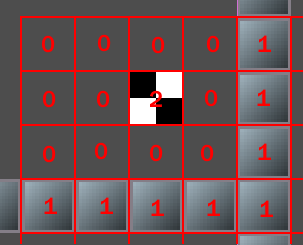
\includegraphics[width=0.8\textwidth]{figures/tilemap.png}
    \caption{Classifying tiles by type}
    \label{fig:tilemap}
\end{figure}

From a technical perspective, 2D platformers require fewer computational resources than 3D games, enabling me to focus more processing power on the machine learning components rather than graphics rendering. 
Godot's excellent 2D capabilities made this genre particularly suitable, as the engine provides robust tools for sprite animation, tilemap management, and physics-based movement.
Additionally, platformers offer clear, discrete states and actions that translate well to reinforcement learning problems. 
The character can move left, right, jump, or perform other specific actions, while the game state can be represented efficiently for the ML model to process.
This clarity in the action space makes platformers an excellent testbed for AI development, as the model must learn fundamental gaming concepts like obstacle avoidance, timing, and spatial navigation.
The tile-based structure also facilitates procedural level generation, allowing me to create varied environments for training the AI without manually designing each level. 
This was particularly important for developing robust models that could generalize across different scenarios rather than overfitting to specific level layouts.

I decided to design the game around a clear, measurable objective: completing a time-based obstacle course. This design choice was deliberate as it provides several advantages for both gameplay and AI development.
From a gameplay perspective, a timed obstacle course offers an intuitive goal that requires no elaborate explanation - players simply need to reach the end as quickly as possible. 
This straightforward objective creates natural replay value as players (human or AI) attempt to optimize their route and execution to achieve faster completion times.
From a machine learning standpoint, this objective is ideal because it creates a well-defined reward function where success can be quantified precisely through time measurements. 
The faster an agent completes the course, the better its performance, providing a clear optimization target for reinforcement learning algorithms.
This design also allows for incremental learning progression. An AI agent can first learn the fundamental task of reaching the goal, then gradually optimize for speed - mirroring how human players typically approach such challenges. 
The continuous nature of the time metric (as opposed to binary success/failure) gives the learning algorithm more nuanced feedback about small improvements in performance.
Additionally, timed courses naturally incorporate key platforming challenges like precise jumping, obstacle avoidance, and route optimization, creating a rich environment for AI learning while remaining accessible to human players for comparison.

\section{Spriting and Graphics}
A small part of this project involves the creation of graphics, so we can see what is going on. In 2D games these are referred to as sprites.
For the graphical elements of the game, I opted to create all assets using Aseprite, a specialized pixel art editor. This decision aligned perfectly with both the technical requirements of the project and the aesthetic direction I wanted to pursue.
I deliberately chose a pixel art style for several reasons. 
First, the simplicity of pixel graphics reduced development time, allowing me to focus more on the AI components that were the primary focus of my research. 
Second, pixel art's grid-based structure naturally complemented the tile-based nature of the platformer, creating visual coherence between the mechanics and aesthetics. 
Finally, the minimalist style ensured that game elements remained visually distinct and easily recognisable.
Using Aseprite, I created character sprites for the player character and AI character, as well as tiles for terrain and the finish line.
I maintained a consistent color palette throughout to ensure visual harmony, limiting myself to a small set of colors that clearly differentiated between game elements while providing adequate contrast.
For creating the user interface I used two fonts: PressStart2P, and the default Godot font provided with the engine. Both are open source and free to use.

\section{Building a Basic Game Environment}

My first task was to build a basic game environment within Godot that could then be built further upon.
This consists of:
\begin{itemize}
    \item \textbf{Player Character}: I implemented a character with basic movement controls including running left/right, jumping, and falling with appropriate physics, using Godot's built in 2D physics system.
    \item \textbf{Camera}: The game's camera is a Camera2D node that remains static providing a view of the whole map.
    \item \textbf{Tile Based Map}: I created a tilemap system using Godot's TileMapLayer node, allowing me to construct levels from reusable tiles representing walls, floors and ceilings.
    \item \textbf{Kill Plane}: At the bottom of the map, there is a player collidable box that will reset their position if it is touched. This ensures that the player cannot fall out of the map endlessly.
    \item \textbf{Finish Line and Timer}: Each map contains a finish line tile. As soon as the player is instantiated, their timer starts and will stop once they touch the finish line.
\end{itemize}

\begin{figure}[H]
    \centering
    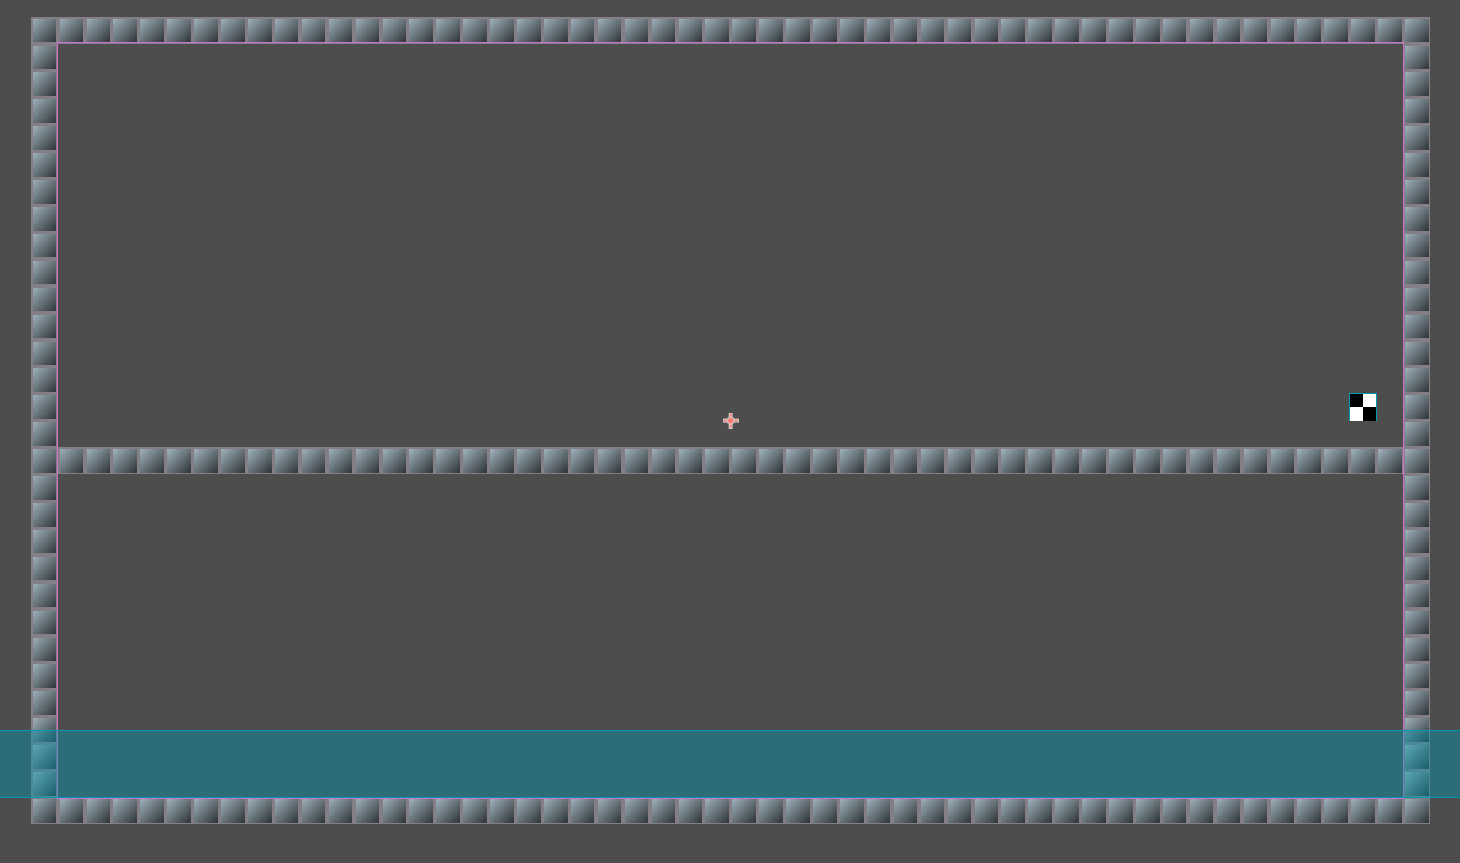
\includegraphics[width=0.8\textwidth]{figures/godot_environment_basic}
    \caption{Basic Godot game environment}
    \label{fig:godot_environment_basic}
\end{figure}

Godot's node based architecture allowed me to neatly lay these all out.

\begin{figure}[H]
    \centering
    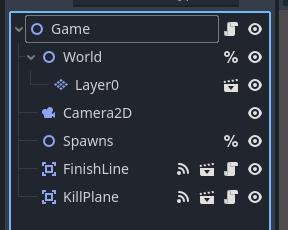
\includegraphics[width=0.8\textwidth]{figures/godot_nodes_basic.png}
    \caption{Environment's node hierarchy}
    \label{fig:godot_nodes_basic}
\end{figure}

\section{State Observation System}

For the reinforcement learning agent to make informed decisions, it needs to perceive its environment effectively. 
This required designing an observation system that captures relevant environmental information while maintaining computational efficiency.

\subsection{Observation Scope and Representation}

While capturing the entire environment state would provide the agent with complete information, such an approach proved prohibitively expensive from a computational perspective. A full environment representation would:

\begin{itemize}
    \item Significantly increase the input dimensionality of the neural network
    \item Require substantially more training time to converge
    \item Demand greater memory resources during both training and inference
    \item Scale poorly with larger environment sizes
\end{itemize}

After experimentation with various observation window sizes, I determined that a 7×7 grid centered on the player offered an optimal balance between environmental awareness and computational efficiency. 
This window size provides sufficient context about nearby obstacles, pathways, and goals while keeping the state representation compact and manageable. 
The constrained field of view also encourages the agent to develop more generalizable navigation strategies rather than memorizing specific map layouts, potentially improving transfer learning capabilities across different environments.
The agent perceives a 7×7 grid centered on its position, providing sufficient contextual awareness of the immediate surroundings.

This observation window uses a simple numerical encoding scheme:
\begin{itemize}
    \item \textbf{0}: Empty space / traversable areas 
    \item \textbf{1}: Player character (Always at the centre of the grid)
    \item \textbf{2}: Finish line
    \item \textbf{3}: Walls / non-traversable terrain
\end{itemize}

\begin{figure}[H]
    \centering
    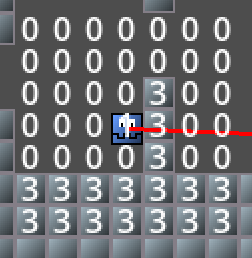
\includegraphics[width=0.8\textwidth]{figures/observation_window}
    \caption{Visualisation of the observation window}
    \label{fig:observation_window}
\end{figure}

\subsection{Implementation Mechanics}

The observation mechanism operates on each frame update, scanning the surrounding tiles relative to the agent's position. 
For each coordinate within the 7×7 grid, the system queries the tilemap to determine the tile type at that location. 
This information is then encoded according to the numerical scheme and assembled into a two-dimensional array.
This process is run twice, once for the initial observation, and again for the second observation used alongside the reward.

This representation offers several advantages:
\begin{itemize}
    \item \textbf{Translation invariance}: The agent learns based on relative positions rather than absolute map coordinates
    \item \textbf{Computational efficiency}: The fixed-size input simplifies network architecture and reduces processing requirements
    \item \textbf{Informational clarity}: The categorical encoding provides clear distinctions between critical environmental features
\end{itemize}

Once constructed, this state representation is transmitted to the reinforcement learning model, which uses it as input for determining the next optimal action. 

\section{Determining reward}
Designing an effective reward function was critical for the reinforcement learning agent's success. After extensive experimentation, I implemented a straightforward distance-based reward mechanism that provides immediate feedback after each action:

\begin{itemize}
    \item \textbf{+1 reward} when the agent moves closer to the finish line
    \item \textbf{-1 penalty} when the agent moves further from the finish line
    \item \textbf{+1 additional reward} upon reaching the goal
\end{itemize}

This reward function is run once each frame, alongside the second observation, after the model has made an action.

This simple approach encourages the agent to make continuous progress toward the objective while maintaining computational efficiency. 
The reward function balances immediate guidance with the freedom to discover optimal paths independently.
During development, I explored several alternative reward structures, including proportional multipliers (×1.2/×0.8) and larger magnitude rewards (+600 for goal completion, -300 for falling). 
However, these higher values led to training instability, causing the model to struggle with convergence. The proportional multipliers proved beneficial and were retained, while the reward magnitudes were scaled back to ±1 to ensure stable learning.
I also experimented with line-of-sight rewards using raycasting techniques, where the agent would receive additional rewards when establishing visual contact with the goal. 
After testing, this approach was ultimately not incorporated into the final implementation as it did not significantly improve performance while adding computational overhead.

A significant limitation of this reward structure is that it discourages exploratory backtracking, effectively requiring level designs to maintain a linear progression toward the goal. 
This constraint arises because the agent receives consistent penalties when moving away from the finish line, even when such movements might be strategically necessary to navigate complex environmental features. 
While this simplifies the learning process for straightforward courses, it potentially limits the agent's ability to discover optimal solutions in more complex, non-linear environments where temporary retreat may be advantageous.

\section{Implementing Networking}

To facilitate communication between the Godot game environment and the Python-based reinforcement learning model, I developed a robust networking system using TCP sockets and JSON encoding. This approach allows the game state to be effectively transmitted to the model for processing, and action decisions to be received back for execution within the game environment.

\subsection{Communication Protocol Design}

After evaluating several options for inter-process communication, I selected a TCP socket-based approach with JSON encoding for several key reasons:

\begin{itemize}
    \item \textbf{Reliability}: TCP's connection-oriented nature ensures that no state observations or action commands are lost during transmission
    \item \textbf{Flexibility}: JSON encoding provides a structured yet adaptable format for representing complex game state information
    \item \textbf{Cross-platform compatibility}: The socket-based approach works seamlessly across different operating systems
    \item \textbf{Low implementation overhead}: Both Godot and Python offer built-in libraries for TCP communication without requiring additional dependencies
\end{itemize}

To implement this, I used the \textit{socket} library on the python side, and a \textit{StreamPeerTCP} node on the Godot side.

\subsection{Operational Modes}

The Python component of the system was designed with two distinct operational modes:

\begin{itemize}
    \item \textbf{Training Mode}: Incorporates epsilon-greedy exploration strategies and periodically saves model checkpoints to preserve training progress. This mode focuses on model improvement through experience gathering and optimization.
    \item \textbf{Play Mode}: Loads the latest saved checkpoint and plays deterministically with epsilon set to zero, demonstrating the current capabilities of the trained model without further exploration.
\end{itemize}

\subsection{Communication Cycle Implementation}

The core networking loop on the Godot side follows a structured pattern of state transmission and action reception:

\begin{enumerate}
    \item First, the game engine calculates and sends the reward from the previous action along with the current state observation
    \item It then awaits confirmation that the Python script is ready for the next cycle
    \item Upon confirmation, the game sends a fresh observation of the current environment state
    \item Finally, it receives the model's selected action (encoded as an integer: 0 for left movement, 1 for right movement, 2 for jump) and executes this action within the game environment
\end{enumerate}

This communication cycle repeats once each frame during gameplay, maintaining a consistent feedback loop between the game environment and the learning model. 
The implementation ensures that state observations, rewards, and actions are synchronized properly, preventing timing issues that could otherwise lead to misaligned learning experiences.

The code excerpt below illustrates the essential communication pattern:

\singlespaced
\begin{verbatim}
# Transmit previous reward and current state
var model_reward : float = reward()
peer.put_float(model_reward)
peer.poll()
var next_state : Dictionary = observe()
var next_state_encoded : PackedByteArray = JSON.stringify(next_state).to_utf8_buffer()
peer.put_data(next_state_encoded)
peer.poll()

# Await ready signal from Python
peer.poll()
var _isready : String = peer.get_string(5)

# Reset reward flags
deathPenalty = false
winReward = false

# Send observation for decision making
var visibleTiles : Dictionary = observe()
var visibleTilesEncoded : PackedByteArray = JSON.stringify(visibleTiles).to_utf8_buffer()
peer.put_data(visibleTilesEncoded)
peer.poll()

# Receive and execute model's action decision
peer.poll()
var model_action : int = peer.get_u8()
action(delta, model_action)
\end{verbatim}
\doublespaced

This networking implementation provides the critical infrastructure that allows the reinforcement learning agent to interact with the game environment, facilitating the entire learning process.
\section{Implementing the Model}

For the reinforcement learning component, I implemented a Deep Q-Network (DQN) architecture with convolutional layers to process the spatial information from the game environment.

\subsection{Model Architecture}

After considering various neural network architectures, I selected a convolutional DQN model that could efficiently process the 2D grid observation data from the game environment:

\begin{itemize}
    \item \textbf{Input Layer}: Accepts the 7×7 grid observation (49 values) reshaped into a 2D format
    \item \textbf{Convolutional Layer}: A 2D convolutional layer with 16 filters, kernel size of 3×3, stride of 1, and padding of 1, enabling the network to detect spatial patterns in the environment
    \item \textbf{Hidden Layers}: Two fully-connected layers with 128 neurons each and ReLU activation functions
    \item \textbf{Output Layer}: A fully-connected layer with 4 outputs corresponding to the possible actions (move left, move right, jump, do nothing)
\end{itemize}

The convolutional layer was particularly important for this implementation as it allows the model to recognize patterns in the spatial arrangement of walls, empty spaces, and the goal within the observation window. 
This spatial awareness is critical for navigating the platformer environment effectively.

\subsection{Training Algorithm}
W
I implemented a standard Q-learning algorithm with experience replay and a target network for stable training:

\begin{itemize}
    \item \textbf{Epsilon-greedy Exploration}: Starting with a high exploration rate that gradually decreased over time, balancing exploration of new strategies with exploitation of learned knowledge
    \item \textbf{Target Network}: A separate network with parameters periodically updated from the main network to provide stable Q-value targets during training
    \item \textbf{Optimizer}: Adam optimizer with a learning rate of 0.001, selected for its adaptive learning rate capabilities
    \item \textbf{Loss Function}: Mean Squared Error between predicted Q-values and target Q-values
\end{itemize}

\subsection{Training Process}

The training process operated on a cycle-by-cycle basis with the game environment:

\begin{enumerate}
    \item Receive the current state observation from the Godot environment
    \item Select an action using the epsilon-greedy policy
    \item Send the selected action to the game environment for execution
    \item Receive the reward and next state observation
    \item Update the Q-network using the Bellman equation
    \item Periodically update the target network parameters
\end{enumerate}

During training, the epsilon value (controlling exploration vs. exploitation) decayed from an initial value of 0.9 to a minimum of 0.1, 
allowing the agent to gradually transition from predominantly random exploration to informed decision-making based on learned values.
